Przez ostatnie lata dziedzina cyfrowego przetwarzania obrazu bardzo prężnie rozwijała się. W wyniku tego aktualnie dostępnych jest wiele usług pozwalających na uzyskiwanie danych z obrazu. W przypadku tej pracy najbardziej użytecznymi informacjami jest lokalizacja oraz identyfikacja twarzy.
Na rysunku \ref{tab:systemy} przedstawiono cechy kilku wybranych systemów, stworzonych przez jedne z największych firm zajmujących się technologiami informatycznymi na świecie.

\begin{table}[H]\label{tab:systemy}
	\centering
	\caption{Dostępne systemy przetwarzania obrazu}
	\scalebox{0.75}{
	\begin{tabular}{|c|c|c|c|c|c|c|}
  		\hline 
  		 & \bfseries OpenCv & \bfseries Azure CS & \bfseries AWS Rekognition & \bfseries Google & \bfseries face recognition & \bfseries open face\\
  		\hline
  		\bfseries Detekcja twarzy &tak&tak&tak&tak&tak&tak\\
  		\hline
  		\bfseries Identyfikacja twarzy &tak&tak&tak&nie&tak&tak\\
  		\hline
  		\bfseries Rozpoznawanie emocji &nie&tak&nie&nie&nie&nie\\
  		\hline
  		\bfseries SDK &tak&tak&tak&tak&Python&Python\\
  		\hline
  		\bfseries API &nie&tak&tak&tak&nie&nie\\
  		\hline
  		\bfseries licencja &open source&płatna/demo&płatna/demo&płatna/demo&open source&open source\\
  		\hline
  	\end{tabular}
  	}
\end{table}
Zgodnie ze wzrostem popularności usług chmurowych, aktualnie dostępnych jest wiele usług rozpoznawania twarzy, które początkowo były dostępne za pomocą API(Application Programming Interface). Z czasem większość z nich udostępniła również SDK(Software Development Kit) dla najbardziej popularnych języków (między innymi C\#, Java, Python). OpenCv \cite{opencv_doc} jest podstawową open sourcową bibliotekę pozwalającą na identyfikację twarzy. Większość darmowych rozwiązań dostępnych jest na platformie GitHub:
\begin{itemize}
\item face\_ recognition \cite{face_reco_github},
\item open face \cite{open_face}.
\end{itemize}
Niestety żadna z nich nie mogła równać się dojrzałością podobną do OpenCv, a na dodatek większość z nich
można wykorzystać jedynie tworząc oprogramowanie w języku Python.

Poza usługami przedstawionymi w tabeli \ref{tab:systemy}, równie ciekawym rozwiązaniem, aczkolwiek znacznie bardziej rozbudowanym i czasochłonnym jest wykorzystanie Tensorflow \cite{tensorflow} (framework do machine learningu) w celu zbudowanie własnej implementacji sieci neuronowej rozpoznającej twarze.
Podstawowym frameworkiem, o którego użyciu zadecydowano zostało OpenCv. Za wyborem tej biblioteki przemawiała licencja open source, dojrzałość frameworku oraz liczne źródła wiedzy o implementacji. Podstawowe dostępne funkcje i zastosowania opisano w rozdziale \ref{s:open_cv}.

W celu możliwości porównania rozwiązań lokalnych i chmurowych za drugi obiekt badań obrano usługę Azure Cognitive Services \cite{acs_doc}, którą szerzej opisano w rozdziale \ref{azurecs}. O wyborze tego rozwiązania zadecydowała rozbudowana dokumentacja usługi oraz licencja studencka umożliwiająca darmowe wykorzystanie usługi przy zwiększonych limitach zapytań.

\section{Open Cv} \label{s:open_cv}
OpenCv (Open Source Computer Vision Library) jest open sourcową biblioteką napisaną w języku C. Udostępniono liczne interfejsy biblioteki pozwalające na pracę z nią miedzy innymi w języku C++ i Python. Biblioteka wspiera systemy operacyjne Linux oraz Windows. Biblioteka została ukierunkowana na przetwarzanie obrazu w czasie rzeczywistym. W licznie udostępnionych funkcjach można znaleźć moduły pozwalające na detekcję i rozpoznawanie twarzy na obrazie, które zostały szerzej opisane w kolejnym punkcie.

\subsection{Rozpoznawanie twarzy}
Przed zidentyfikowaniem tożsamości, należy najpierw rozwiązać problem detekcji twarzy. Podstawowym sposobem detekcji twarzy wykorzystywanym przez OpenCv jest kaskadowy klasyfikator Haar'a oparty o cechy Haar'a opisane w rozdziale \ref{haar}. Do innych dostępnych rozwiązań wykorzystanych do stworzenia aplikacji należy wytrenowany model głębokiej sieci neuronowej przygotowany przez autorów biblioteki.

\subsubsection{Eigenfaces} \label{s:eigen}
Eigenfaces \cite{opencv_doc} nazywany jest również algorytmem twarzy własnych. Głównym postanowieniem algorytmu jest to że nie wszystkie wymiary w zbiorze danych są równie ważne, więc należy znaleźć elementy, w których występuje największa zmienność bo to one mają największą wartość informacyjną. Obraz o wymiarze $p$x$q$ tworzy wektor o wymiarze $m=pq$, więc przykładowo dla wymiarów 100x100 uzyskuje się wektor o wymiarze 10 000. W celu ekstrakcji głównych składowych wykorzystano analizę głównych składowych (ang principal component analysis, PCA \cite{pca_lda}), która potrafi przekształcić wielowymiarowy zbiór danych skorelowanych w mniejszy zbiór danych nieskorelowanych. Informację o sposobie działania algorytmu zaczerpnięto z dokumentacji \cite{opencv_doc}.

Działanie algorytmu:
\begin{enumerate}
\item Wyznaczenie wartości średniej $\mu$. Weźmy $n$ wektorów $x_{i}$ reprezentujących obrazy przedstawiające twarz.
\begin{equation}
\mu=\frac{1}{n}\sum_{i=1}^{n}x_{i}
\end{equation}
\item Obliczenie wartości macierzy kowariancji $S$
\begin{equation}
S=\frac{1}{n}\sum^{n}_{i=1}(x_{i}-\mu)(x_{i}-\mu)^{T}
\end{equation}
\item Oblicz wartości eigena $\lambda_{i}$ i wektory eigena $\nu_{i}$ z \begin{equation}
S\nu_{i}=\lambda_{i}\nu_{i},i=1,2,...,n
\end{equation}
\item Posortuj wektory eigena według ich wartości eigena. Główne składowe $k$ są wektorami eigena odpowiadającymi $k$ największym wartościom eigena.
\item Oblicz macierz zawierającą $k$ głównych składowych obserwowanych wektorów $x$.
\begin{equation}
y=W^{T}(x-\mu)
\end{equation}
gdzie $W=(\mu_{1},\mu_{2},...,\mu_{l})$
\end{enumerate}

Identyfikacja twarzy algorytmem Eigenfaces polega na wykonaniu kroków:
\begin{enumerate}
\item Wyznaczenie głównych składowych dla wszystkich obrazów uczących.
\item Wartość głównych składowych zostaje wyznaczona dla badanego zdjęcia.
\item Dla obrazu wejściowego zostaje wyznaczony wektor najbliższy do wartości obliczonych podczas trenowania..
\end{enumerate}

\subsubsection{Fisherfaces} \label{fisher}
Algorytm Fisherfaces \cite{opencv_doc} opiera się na liniowej analizie dyskryminacyjnej (ang. latent dirichlet allocation, LDA \cite{pca_lda}) i polega na wyznaczeniu wektora cech pozwalającego na rozdzielenie obiektów przynależnych do różnych klas. Przez klasę rozumie się zbiór obrazów przedstawiających tego samego użytkownika. Problem sprowadza się do wyznaczenia wektora, który stanowi przybliżoną granicę między dwiema klasami obiektów, jednak można go uogólnić do problemu wieloklasowego. W efekcie podobne klasy powinny być ze sobą ściśle połączone, podczas gdy różne klasy znajdują się jak najdalej od siebie. Opis działania algorytmu zaczerpnięto z dokumentacji \cite{opencv_doc}.

Działanie algorytmu:
\begin{enumerate}
\item Weźmy wektor $X$ złożony z próbek należących do $c$ klas
\begin{equation}
X=\{X_{1},X_{1},...,X_{c}\}
X_{i}=\{x_{1},x_{1},...,x_{c}\}
\end{equation}
\item Oblicz macierz rozproszenia wewnątrzklasowego $S_{B}$ i macierz średniego rozproszenia wewnątrzklasowego $S_{W}$
\begin{equation}
S_{B}=\sum_{i=1}^{n}N_{i}(\mu_{i}-\mu)(\mu_{i}-\mu)^{T}
\end{equation}
\begin{equation}
S_{W}=\sum_{i=1}^{n}\sum_{x_{j}\in X_{i}}(x_{j}-\mu_{i})(x_{j}-\mu_{i})^{T}
\end{equation}
gdzie $\mu$ oznacza całkowitą średnią:
\begin{equation}
\mu=\frac{1}{N}\sum_{i=1}^{N}x_{i}
\end{equation}
a $\mu_{i}$ średnią klasy $i\in \{1,...c\}$
\begin{equation}
\mu_{i}=\frac{1}{|X_{i}|}\sum_{x_{j}\in X_{i}}x_{j}
\end{equation}
\item Znajdź wektory bazowe $W$ gdzie $S_{W}$ jest zminimalizowane a $S_{B}$ zmaksymalizowane
\begin{equation}
W_{optymalne}=\frac{\vert W^{T}S_{B}W\vert }{\vert W^{T}S_{W}W\vert }
\end{equation}
\item Rozwiązanie sprowadza się do obliczenia wartości eigena (rozdział \ref{s:eigen})
\begin{equation}
S_{B}\nu_{i}=\lambda_{i}S_{W}\nu_{i}
\end{equation}
\begin{equation}
S_{W}^{-1}S_{B}\nu_{i}=\lambda_{i}\nu_{i}
\end{equation}
\end{enumerate}

Identyfikacja twarzy algorytmem FisherFaces polega na wykonaniu kroków:
\begin{enumerate}
\item Wyznacz wartość twarzy w przestrzeni LDA.
\item Znajdź najbliższego sąsiada w macierzy $W$.
\end{enumerate}

\subsubsection{Local Binary Patterns Histograms} \label{lbph}
Algorytm LBPH \cite{opencv_doc}\cite{lbph} (ang. Local Binary Patterns Histograms, lokalne histogramy binarne) w odróżnieniu od holsitycznego podejścia w Eigenfaces i Fisherfaces algorytm lbph wykorzystuje lokalne cechy przetwarzanych obiektów. Głównym założeniem algorytmu jest wyznaczenie ciągu binarnego dla każdego piksela zdjęcia. Proces zaczyna się przez przyjęcie rozmiaru struktury o wymiarze $X$x$X$ px (np. 3x3 px). Weź piksel jako centralny punkt struktury i zastosuj thresholding binarny dla sąsiadujących z nim pikseli mieszczących się w strukturze. Jeśli wartość piksela jest większa lub równa wartości centralnego piksela to jego nowa wartość to 1. W przeciwnym przypadku piksel otrzymuje wartość 0. Przykładową operację przedstawiono na rysunku \ref{fig:lbph_thresh}.
\begin{figure}[H]
	\centering
	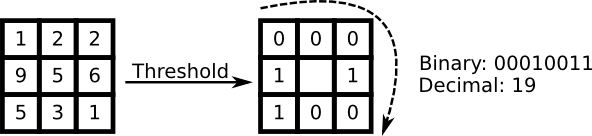
\includegraphics[scale=1.0]{lbph_threshold.png}
		\captionsource{Wyznaczenie lokalnego binarnego wzorca piksela dla struktury 3x3 px}{Dokumentacja OpenCv \cite{opencv_doc}}
	\label{fig:lbph_thresh}
\end{figure}
W ten sposób dla każdego piksela wyznaczana jest wartość $p$ znakowego binarnego ciągu nazywanego lokalnym binarnym wzorcem.

W ogólności wartość funkcji LBP dla piksela o współrzędnych $(x_{c},y_{c})$ wyznacza się następująco:
\begin{equation}
LBP(x_{c},y_{c})=\sum_{p=0}^{p-1}2^{p}S(i_{p}-i_{c})
\end{equation}
gdzie $p$ jest rozmiarem rozpatrywanego sąsiedztwa o środku w punkcie $(x_{c},y_{c})$, jasności o wartości $i_{c}$ i jasności dla $n$-tego piksela $i_{n}$. $s(x)$ jest funkcją znaku zdefiniowaną jako:
\begin{equation}
s(x) = \left\{ \begin{array}{ll}
1 & \textrm{ dla $x>0$}\\
0 & \textrm{ pozostałe}
\end{array} \right.
\end{equation}
Implementacja algorytmu sprowadza się do podzielenia obrazu wejściowego na $m$ regionów i wyznaczenie wartości LBP dla każdego z nich. Następnie wyznaczany jest histogram wyliczonych wartości.

Identyfikacja twarzy algorytmem LBPH polega na wykonaniu kroków:
\begin{enumerate}
\item Wyznacz wektora histogramów dla próbki wejściowej.
\item Porównaj wektor z wektorami obrazów użytych podczas uczenia sieci.
\item Odpowiedź to etykieta wektora najbliższego sąsiada.
\end{enumerate}

\section{Azure Cognitive Services}\label{azurecs}
Cognitive Services jest częścią platformy Azure stworzonej przez Microsoft. Usługa jest płatna, ale w przypadku użytku na potrzeby studenckie przyznawany jest darmowy dostęp na ograniczony czas. Cognitive Services zajmuje się rozwiązywaniem problemów biznesowych dzięki sztucznej inteligencji. Do dostępnych modułów między innymi należą:
\begin{itemize}
\item obraz- algorytmy przetwarzania obrazów umożliwiające inteligentne identyfikowanie, podpisywanie i moderowanie grafik,
\item mowa- konwertowanie wypowiedzi audio na tekst, weryfikacja głosowa,
\item język- przetwarzanie języka naturalnego.
\end{itemize}
Na cele tego projektu wykorzystano moduł dotyczący przetwarzania obrazu, a dokładniej funkcjonalność wykrywania i rozpoznawania twarzy. Producent zadbał o możliwość integracji z większością popularnych języków programistycznych poprzez udostępnienie paczek deweloperskich. W przypadku braku SDK(Software Development Kit) dla wybranego języka istnieje możliwość skorzystania z udostępnionego REST Api. Na stronie producenta można znaleźć obszerną dokumentację \cite{acs_doc} oraz tutoriale.

\subsection{Detekcja twarzy}
Detekcja twarzy opiera się o pojedyncze zapytane do Api Azure'a. Dobierając odpowiednie parametry wejściowe klient może uzyskać dodatkowe informacje związane z przesłanym zdjęciem. W podstawowym przypadku odpowiedź serwisu ogranicza się do przydzielenia identyfikatora dla twarzy oraz obszaru zawierającego twarz w postaci JSON'a.

\subsection{Rozpoznawanie twarzy}
Na potrzeby rozpoznawania twarzy stworzono funkcja LargeGroup, która odpowiada za zarządzanie grupami ludzi/profili. Użytkownik może dodać dowolną ilość osób do grupy, a następnie przypisać wybrane zdjęcia do tożsamości.Na podstawie utworzonej grupy zostaje stworzony model umożliwiający rozpoznawania tożsamości osób w niej zawartej. Sposób wykorzystania tej usługi został znacznie szerzej opisany w rozdziale \ref{trenowanie_azure}. Sposób działania usługi bazuje nauczeniu maszynowym.

\section{AWS Rekognition}
Usługa Rekognition jest odpowiednikiem Azure Cognitive Services ograniczonym do rozwiązań związanych z przetwarzaniem obrazu i video. Do wielu dostępnych funkcji należy analiza obrazu, detekcja twarzy i tekstu, porównywanie oraz rozpoznawanie twarzy. Dla wybranych języków programistycznych udostępniono SDK(Software Development Kit) oraz obszerną dokumentację z licznymi przykładami kodu.
